% SPDX-FileCopyrightText: 2026 Mert Torun
% SPDX-License-Identifier: CC-BY-4.0
%
% Frames of the deck of the talk at the VIMS-Workshop 2026, input by
% presentation.tex; the handout is written separately. Statements follow the
% revised edition of the research report (report/), cited by section.

% ---- Title ---------------------------------------------------------------
\begin{frame}[plain]
  \titlepage
  \vspace{-1.5em}
  \begin{center}\scriptsize
    Paper: Working Paper in K\"olner Beitr\"age zur technischen Informatik 2/2026, published, \url{https://doi.org/10.57684/COS-1494}\\[2pt]
    {\color{inkgray}The deck as presented on 22~May 2026 is not archived; these are its sources, revised in October 2026.}
  \end{center}
\end{frame}

% ---- Motivation ----------------------------------------------------------
\begin{frame}{Motivation: ageing safety-critical electronics}
  \begin{itemize}
    \item The anti-skid (wheel-slide protection) system of this case has been in service in European urban rail since the early 1990s; its test-diagnosis module is built on the obsolete Intel MCS-48 family (report, Ch.~1).
    \item As the parts become unobtainable, the choice is between replacing the system and a targeted \emph{board-level retrofit}, which can defer cost and avoid the embodied emissions of new subsystems; the report argues this advantage and does not quantify it (Sec.~5.5.3).
    \item A retrofit has to show \alert{functional equivalence} with the original under contemporary safety standards.
  \end{itemize}
  \revised{the deployment is limited to the documented case; the cost and carbon advantage is marked as argued, not quantified.}
\end{frame}

% ---- The gap -------------------------------------------------------------
\begin{frame}{The question}
  \begin{itemize}
    \item Prior work covers the \emph{formal verification of new} safety-critical designs and \emph{hardware-in-the-loop} testing of braking and anti-skid control units.
    \item The author is not aware of an established method for verifying functional equivalence \alert{at the board level} when a legacy microcontroller is replaced by FPGA emulation (report, Ch.~1).
  \end{itemize}
  \vfill
% SPDX-SnippetBegin
% SPDX-SnippetCopyrightText: 2026 Mert Torun
% SPDX-License-Identifier: CC-BY-NC-ND-4.0
% SPDX-SnippetComment: The research question of the paper, quoted from page 3 of the deposited file; licensed like the paper. See NOTICE.
  \begin{block}{Research question}
    How can functional equivalence in safety-critical hardware retrofits be rigorously demonstrated through structured, standards-aligned verification?
  \end{block}
% SPDX-SnippetEnd
  \revised{``no established methodology exists'' is stated as the author's knowledge; the HIL work cited tests control units, not complete braking systems.}
\end{frame}

% ---- Contributions -------------------------------------------------------
\begin{frame}{Contributions, as the revised report states them}
  \begin{enumerate}
    \item \textbf{A documented case:} the retrofit of one test-diagnosis module, from the inherited prototype to the rebuilt unit, with what is and is not documented about its verification.
    \item \textbf{A classification of integration defects:} six defects documented during the rebuild, by type and by how they were found; no single method found all of them.
    \item \textbf{A proposed verification structure:} two layers on the verification side of the V-model, mapped to whole standards; the structure is proposed, not validated.
  \end{enumerate}
  \footnotesize Prior work: S.~Ayoub (2014), M.~Leyer (2023), A.~Dolata, D.~Ostermann and F.~Schiffelers (2023), and a follow-on project (2025); the report credits each (Sec.~1.4).
  \revised{the contributions follow report Sec.~1.4; the claim that each defect was caught by exactly one layer is withdrawn.}
\end{frame}

% ---- Architecture --------------------------------------------------------
\begin{frame}{The retrofit: four boards, two processors}
  \begin{columns}[T]
    \begin{column}{0.56\textwidth}
      \begin{itemize}\small
        \item \textbf{Base Board:} Actel A3P1000 flash FPGA emulating the MCS-48 with the OpenCores \texttt{t48} core, integrated unmodified, and running the original firmware from an external Flash ROM.
        \item \textbf{STM32 Diagnostics Board:} STM32F401RET6 logger behind four SFH601-3 optocouplers (three SPI lines and a reset line) and an isolated DC/DC converter.
        \item \textbf{Upper and LED Boards:} the legacy buttons, the external watchdog and the displays; brown-out supervision on the Base Board.
      \end{itemize}
    \end{column}
    \begin{column}{0.44\textwidth}
      \centering
      \begin{tikzpicture}[font=\scriptsize, node distance=4mm,
        box/.style={draw, rounded corners=2pt, minimum width=2.7cm, minimum height=8mm, align=center}]
        \node[box, fill=ieeeblue!12] (fpga) {FPGA (A3P1000)\\MCS-48 emulation};
        \node[box, fill=accentteal!15, below=of fpga] (stm) {STM32F401RET6\\diagnostics};
        \draw[-{Stealth[length=2mm]}, very thick, densely dashed, red!70!black]
          (fpga) -- node[right=1pt]{\,isolated SPI} (stm);
        \node[below=1mm of stm, text=red!70!black] {\itshape galvanic boundary};
      \end{tikzpicture}
    \end{column}
  \end{columns}
  \medskip
  \footnotesize The boards' design is M.~Leyer's (2023); the parts of the diagnostics board on the Base Board side of the barrier share its supply (report, Secs.~3.1 and 3.3).
  \revised{no firmware size is given, since it is not established; the optocouplers and the single isolated converter are described as fitted; the design is credited.}
\end{frame}

% ---- Methodology ---------------------------------------------------------
\begin{frame}{Two layers on the V-model}
  \begin{columns}[T]
    \begin{column}{0.5\textwidth}
      \begin{itemize}
        \item \textbf{Layer 1, component and interface tests:} white-box and deterministic; is each artefact implemented as specified?
        \item \textbf{Layer 2, system-level tests:} black-box and scenario-based; does the integrated module reproduce the legacy behaviour?
      \end{itemize}
      \medskip
      Both stand on the right arm of the V-model; each is meant to cover what the other cannot observe.
    \end{column}
    \begin{column}{0.5\textwidth}
      \centering
% SPDX-SnippetBegin
% SPDX-SnippetCopyrightText: 2026 Mert Torun
% SPDX-License-Identifier: CC-BY-NC-ND-4.0
% SPDX-SnippetComment: A simplified drawing after Fig. 2 of the paper, page 6 of the deposited file; licensed like the paper. See NOTICE.
      \begin{tikzpicture}[font=\scriptsize, scale=0.8, every node/.style={transform shape},
        b/.style={draw, rounded corners=2pt, minimum width=1.8cm, minimum height=5mm, align=center}]
        \node[b, fill=red!12] (sr) at (0,2) {System Req.};
        \node[b, fill=yellow!18] (md) at (1.1,0.4) {Module design};
        \node[b, fill=gray!18] (im) at (2.2,-0.6) {Impl.};
        \node[b, fill=green!18] (ut) at (3.3,0.4) {Unit/Int.\ (L1)};
        \node[b, fill=ieeeblue!18] (sv) at (4.4,2) {System val.\ (L2)};
        \draw[-{Stealth[length=1.5mm]}] (sr)--(md); \draw[-{Stealth[length=1.5mm]}] (md)--(im);
        \draw[-{Stealth[length=1.5mm]}] (im)--(ut); \draw[-{Stealth[length=1.5mm]}] (ut)--(sv);
        \draw[{Stealth[length=1.5mm]}-{Stealth[length=1.5mm]}, densely dashed, blue!50!black] (sr)--(sv);
      \end{tikzpicture}
% SPDX-SnippetEnd
    \end{column}
  \end{columns}
  \revised{the two layers are described as intended, not as achieved coverage; no requirement list exists for the left arm (report, Sec.~5.4.1).}
\end{frame}

% ---- Layer 1 -------------------------------------------------------------
\begin{frame}{Layer 1: component and interface tests}
  \begin{itemize}
    \item \textbf{VHDL simulation} (ModelSim ME) of the design of 2023: testbenches without assertions, results checked by eye; its NVRAM model ignored the byte-low enable, so defect B1 passed it.
    \item \textbf{JTAG and pin checks} on the Rev~0.0 prototype: device identification and programming over JTAG, pins checked with a toggle design and a multimeter, the Flash programmed through boundary scan.
    \item \textbf{Oscilloscope measurements} of the watchdog reaction and of the frequency sweep, on the Rev~0.0 prototype in 2023, the sweep against the original board.
  \end{itemize}
  \medskip
  \footnotesize The archived simulations and measurements of Layer~1 date from 2023, before the rebuild, and were made by M.~Leyer (report, Secs.~4.2 and 5.1.1).
  \revised{the JTAG checks, the measurements and their dates follow the report; boundary scan is no longer said to have isolated the solder defects.}
\end{frame}

% ---- Layer 2 -------------------------------------------------------------
\begin{frame}[fragile]{Layer 2: system-level tests on a fixture}
  \begin{columns}[T]
    \begin{column}{0.52\textwidth}
      \begin{itemize}\small
        \item Test fixture (\emph{Testkartentester}) of A.~Dolata, D.~Ostermann and F.~Schiffelers (2023), an STM32 Nucleo board and a Python application.
        \item YAML scenarios, linked to the fault cases of the legacy manual by name; the tester checks the displays and marks each case by hand.
        \item Designed to cover fault-memory cycles, the self-test with the sweep, the buttons, power cycles and the diagnostic SPI link.
      \end{itemize}
    \end{column}
    \begin{column}{0.48\textwidth}
      \scriptsize
% SPDX-SnippetBegin
% SPDX-SnippetCopyrightText: 2023 André Dolata, Dennis Ostermann, Francisco Schiffelers
% SPDX-License-Identifier: LicenseRef-third-party
% SPDX-SnippetComment: Adapted from Listing 3 of the test fixture report (dolata2023); see NOTICE.
      \begin{semiverbatim}
- name: Geber 3 - I
  pin_sets: \{18z: 1, 24d: 0\}
  expected_err_code: "31"
  expected_err_seq: "03 31 09"
  del: False
      \end{semiverbatim}
% SPDX-SnippetEnd
      \tiny Adapted from the fixture report, Listing~3.
    \end{column}
  \end{columns}
  \revised{the fixture and the test case are credited; ``covers'' is stated as the design of the suite (report, Sec.~4.3).}
\end{frame}

% ---- Defects -------------------------------------------------------------
\begin{frame}{Six integration defects and how they were found}
  \centering\scriptsize
  \begin{tabular}{@{}l l >{\raggedright\arraybackslash}p{4.2cm} >{\raggedright\arraybackslash}p{4.4cm}@{}}
    \toprule
    \textbf{ID} & \textbf{Class} & \textbf{Found by} & \textbf{Status} \\
    \midrule
    B1 & Logical      & Symptoms on the fixture (L2), cause by debugging & Resolved \\
    B2 & Test fixture & Failed debugger connection to the fixture & Reworked \\
    B3 & Assembly     & Commissioning: oscilloscope, inspection & Reworked \\
    B4 & Firmware     & Freeze: operation of the diagnostics board (2025); overrun: analysis of the firmware of 2023 & Fix applied (firmware of 2023); diagnostic path not verified separately; freeze with the firmware of 2025: no fix documented \\
    B5 & Interface    & Transmitter: simulation testbench (L1); receiver: not recorded & Receiver: fix applied; transmitter: change not documented; diagnostic path not verified separately \\
    B6 & Schematic and layout & Commissioning of the rebuilt unit & Worked around in the FPGA design \\
    \bottomrule
  \end{tabular}
  \par\medskip
  \footnotesize The defects did not come to light in a planned run of the two-layer method, and no single method found all of them (report, Sec.~5.2, Table~5.4).
  \revised{the table of the report replaces that of five defects; B2 concerns the test fixture; the layers that ``caught'' B1 to B5 are corrected.}
\end{frame}

% ---- Evidence ------------------------------------------------------------
\begin{frame}{State of the evidence}
  \begin{itemize}\small
    \item \textbf{Simulation} (2023) and the \textbf{fixture runs} of the follow-on project on the rebuilt unit (2025, no log archived) indicate equivalence of the fault handling.
    \item \textbf{The only measurement against the original board}, the frequency sweep of 2023, shows a deviation at the low end: the emulation ends at about \SI{850}{\hertz}, the original at about \SI{920}{\hertz}. The duration differs too: by design, the emulation's falling sweep ends after about \SI{102}{\milli\second}, where the fixture report gives about \SI{180}{\milli\second} for the frequency changes of the original test card. Both are open.
    \item \textbf{Two deviations by design:} the STORE and RECALL inputs of the system connector (08z, 08d) no longer act on the fault memory, and the added brown-out circuit adds a reset; their relevance in the vehicle is open (report, Sec.~4.6).
    \item Not documented for the rebuilt unit: the self-test, the Test and T\"ur/V buttons, power cycles, the watchdog, the sweep and the brown-out circuit.
  \end{itemize}
  \medskip
  \footnotesize The evidence does not demonstrate equivalence; a logged repetition on the rebuilt unit and a re-measurement of the original board would close the gaps (report, Sec.~5.1.3, Table~5.3).
  \revised{this frame replaces ``three converging lines'', which stated equivalence as demonstrated.}
\end{frame}

% ---- Sweep figure --------------------------------------------------------
\begin{frame}{Frequency sweep: original board and FPGA emulation}
  \centering
  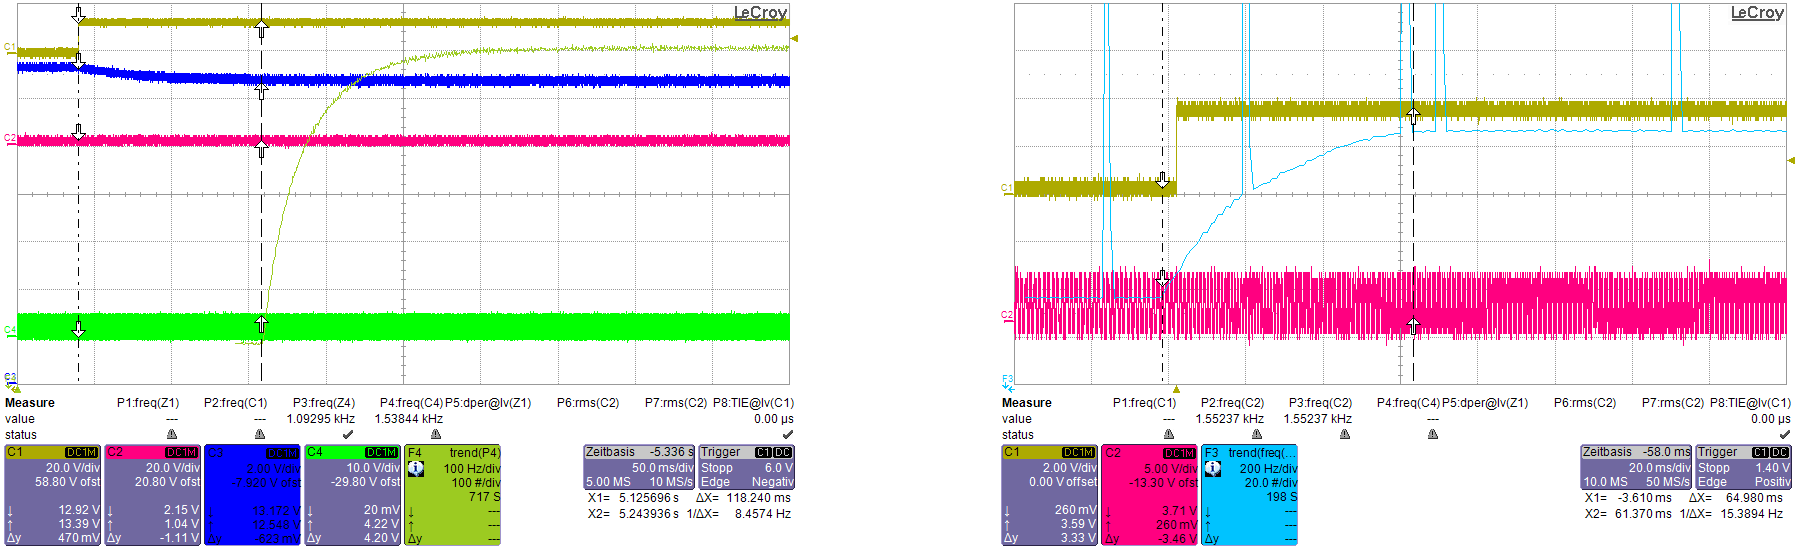
\includegraphics[width=0.49\textwidth]{comp_upsweep.png}\hfill
  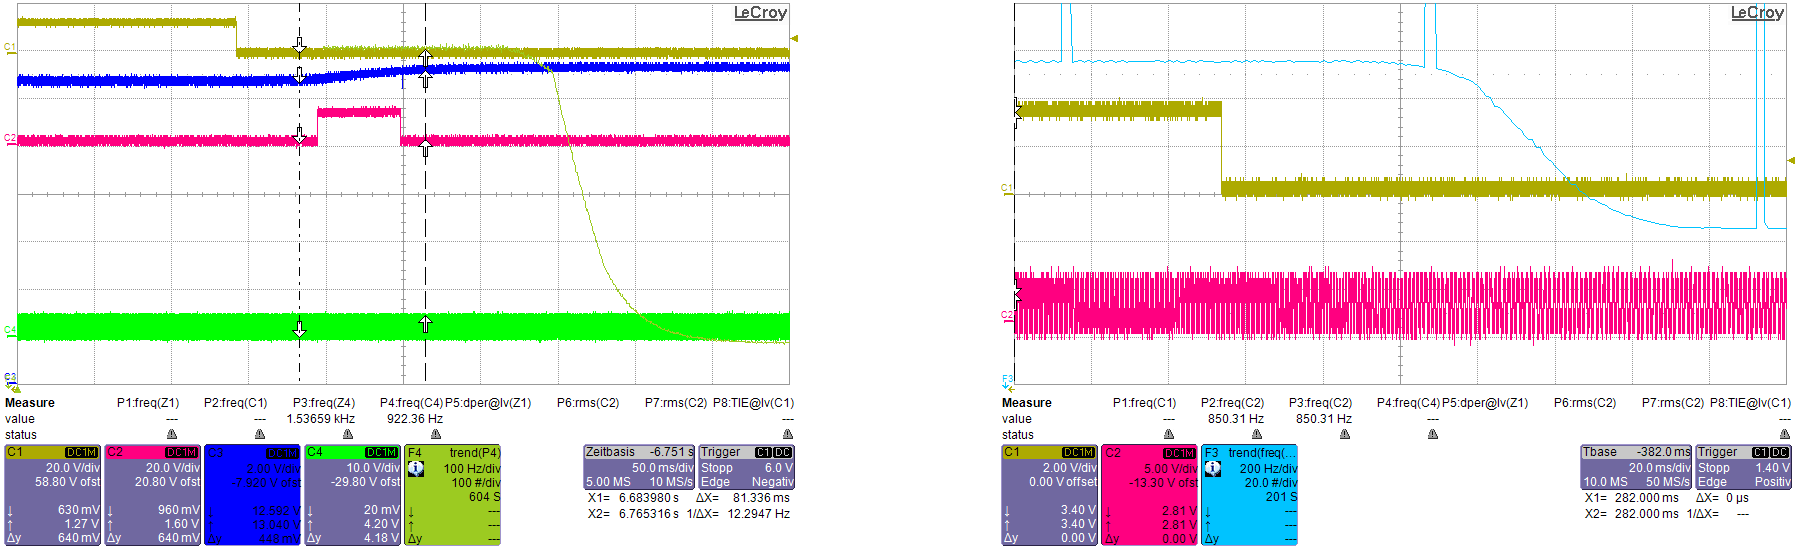
\includegraphics[width=0.49\textwidth]{comp_downsweep.png}
  \par\medskip
  \footnotesize Rising (left) and falling (right) sweeps; in each capture the original board is on the left and the emulation on the right. Captures by M.~Leyer on the Rev~0.0 prototype, July 2023 (his documentation, Figs.~11 and 12). Readouts: the original's low end about \SI{920}{\hertz}, the emulation's about \SI{850}{\hertz} (report, Sec.~5.1.1).
  \revised{the captures are credited and dated, and the frame no longer calls them a result of equivalence.}
\end{frame}

% ---- Standards -----------------------------------------------------------
\begin{frame}{Mapping to standards}
  \centering\small
  \begin{tabular}{@{}lll@{}}
    \toprule
    \textbf{Standard} & \textbf{Scope} & \textbf{Layer} \\
    \midrule
    IEC~61508 & Verification in the safety lifecycle; no SIL assigned & L1 + L2 \\
    EN~50129  & Hardware safety evidence & L1 + L2 \\
    EN~50716  & Software aspects of the modification & L1 + L2 \\
    EN~50155 / EN~61373 & Electronic equipment; shock and vibration & Future \\
    IEEE~1012 & V\&V process; no integrity level assigned & L1 + L2 \\
    \bottomrule
  \end{tabular}
  \vfill
  \footnotesize The layers are mapped to whole standards, not to clauses; the mapping is not an assessment of compliance (report, Sec.~5.4, Table~5.5).
  \revised{the scopes follow Table~5.5 of the report; EN~50716 covers only the software side of the modification.}
\end{frame}

% ---- Limitations ---------------------------------------------------------
\begin{frame}{Scope and limitations}
  \begin{itemize}
    \item \textbf{Diagnostic path (B4, B5):} a fix of the STM32 firmware of 2023 was applied; the rebuilt unit was observed operating as a whole in early 2026; the diagnostic path was not verified separately, and no log or capture was archived.
    \item No hazard analysis, no SIL, no certification and no independent assessment of compliance.
    \item Out of scope: formal methods, structural coverage, accredited environmental testing, full HIL integration.
  \end{itemize}
  \revised{the status of B4 and B5 follows report Sec.~5.3 and Table~5.4; it replaces ``two defects remain open''.}
\end{frame}

% ---- Conclusion ----------------------------------------------------------
\begin{frame}{Conclusion}
  \begin{itemize}
    \item The project indicates, but does not yet demonstrate, that the FPGA retrofit of this module is viable (report, Ch.~6).
    \item No single method found the six defects; component simulation and system tests each saw some, and physical inspection was needed as well.
    \item The two-layer structure can in principle be transferred to other retrofits under IEC~61508; it rests on one case and has not been validated.
  \end{itemize}
  \revised{the conclusion follows the revised report; the deck no longer states that the method demonstrates equivalence.}
\end{frame}

% ---- Future work + thanks ------------------------------------------------
\begin{frame}{Future work and acknowledgements}
  \begin{itemize}
    \item Run the Layer~2 suite on the rebuilt unit with an archived log, repeat the Layer~1 measurements, and measure the original board's sweep again.
    \item Test the diagnostic path with an archived log and move the logging into a non-blocking queue.
    \item Full HIL integration; an IEC~62443 cybersecurity assessment; professionally manufactured boards for accredited environmental tests.
  \end{itemize}
  \vfill
  \footnotesize Acknowledgements: the supervisor, and the contributors to the hardware, firmware and test fixture of the prior and follow-on projects, whom the paper and the report name.
  \vfill
  \begin{center}\structure{\large Thank you; questions welcome.}\end{center}
  \revised{future work follows report Sec.~6.3; the acknowledgement refers to the paper and the report for the names.}
\end{frame}
